\section{Results}
\label{sec:Results}

\subsection{Energy Deposition}
The energy deposition was calcutated for neutron and gamma events for films of thickness of 15 \micron, 25 \micron, 50 \micron, 150 \micron, 300 \micron, 600 \micron, 1 mm and 1 cm (Figure \ref{fig:SimEDepGamma}, \ref{fig:SimEDepNeutron}).  

Photons have a very low probability of interacting in the film due to polymer film being a low z-material.
This is reflected in the majority of the events not interacting at all; about 1 in 10,000 of the events deposit energy in the film as seen in Figure \ref{fig:SimEDepGamma}.
Several classic features of the spectra are apparent on the 1 cm thick thin.
These included the photo-peak in which all of the incident energy of the \iso{Co}{60} is deposited in the film, as well as the individual Compton edges of the two photons fromn \iso{Co}{60}.
These features are not visiable on the measured spectra due to the poor energy resolution of these films.
There is also physical evidance of a lack of a Compton edge on the thinner films, but the films greater than 150 \micron thick show some feature around 0.2 MeV.
Films thinner than 150 \micron show a very small amount of energy deposition that quickly tails off for higher energies, indicating that when a photon interaction occurs in the film the electrons from that interaction leave the film and the only energy deposition occurs from small ionizations as the highly energetic electron leaves the film material.
It is also observed that the thinnest film (15 \micron) has an average energy depostion of around 10 keV, while the 1 cm film has an average energy deposition of around 150 keV.
\begin{figure}[h]
    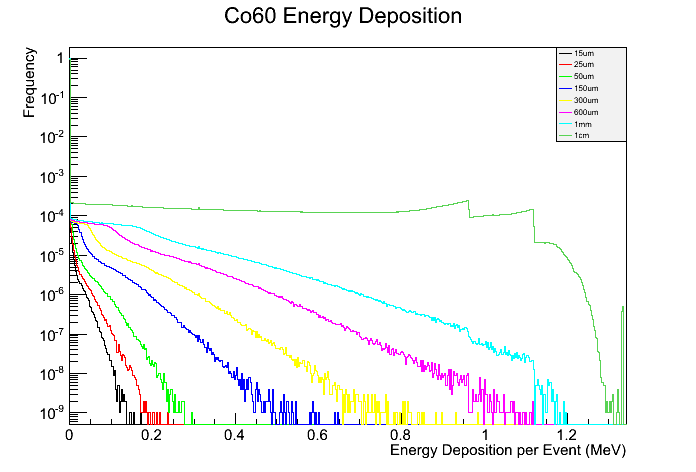
\includegraphics[width=\figurewidth]{Co60EnergyDep}
	\caption{Simulated Energy Depositon for a Single Film (gammas)}
    \label{fig:SimEDepGamma}
\end{figure}
The simulated energy deposition for neutron interactions in thin films is shown in Figure \ref{fig:SimEDepNeutron}.
Several features of the spectra can be immediately noted.
For thick films (1 cm) there is a very high probability that a given event will deposit all of its energy in the film (as expected).
Thinner films have a smaller probability of depositing all of their energy, but this is overshawded by the thick samples when plotted.
It is also intresting to note that it is possible to observe the comparative effects of the the $\alpha$ and \iso{H}{3} in the neutron energy depostion spectra. 
The triton has a much shorter range (\~ 10 \micron in PS \cite{kudo_recoil_1980}) than the $\alpha$ (\~ 60 \micron) so it has a higher probability of depositing all of its energy.
Thus, for energies above 2.73 MeV (the energy of the triton) there is a higher probability of energy energy deposition (by about a factor of 10). These events are still very infrequent compared to the probability of depositing all of the reaction product energy.
Even for the 15 \micron the average energy depostion was above 50\% of the total Q-value of the reaction, and by 200 \micron this average energy deposited approaches 95\% of the total 4.78 MeV.
\begin{figure}[h]
    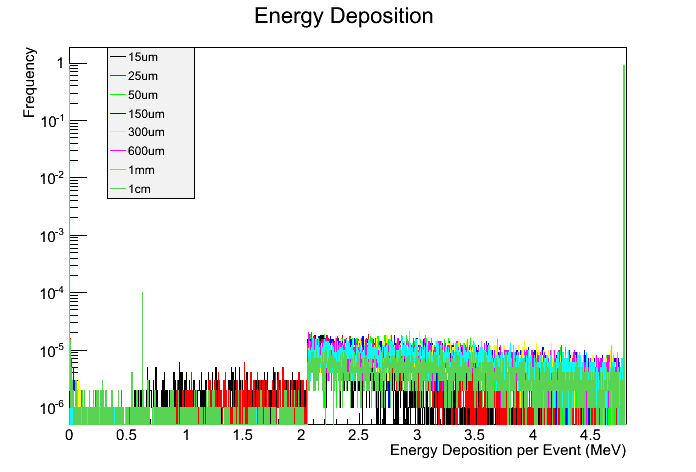
\includegraphics[width=\figurewidth]{NeutronEnergyDep}
	\caption{Simulated Energy Depositon for a Single Film (neutrons)}
    \label{fig:SimEDepNeutron}
\end{figure}

\subsection{Secondary Electron Energy Distribuion}

The distribution of secondary electrons from photon interactions are plotted in Figure \ref{fig:SecElecKinEDist}.
From these results it can be concluded that the it is unlikely (around 1 in 10,000) that an electron will be scattered with the maximum Compton scattering kinetic energy, but rather have an energy somewhat lower than that.
The distribution of secondary electrons from photon interactions is actually very flat, implying that it is likely for the electron from a Compton scattering event to have an energy in the 100's of keV.
The distribution of the next generation of electrons was also calculated, and this distrubiton was also quite entergetic (with a maximum energy corresponding to 0.55 MeV) but with a much large probability of having a collision that produces and electron with a much lower energy.
\begin{figure}[h]
    \centering
    \begin{subfigure}[b]{0.45\figurewidth}
        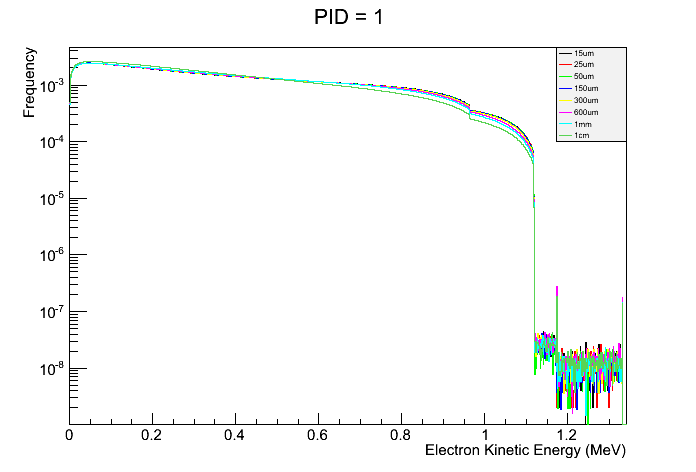
\includegraphics[width=\figurewidth]{Co60_PID1_SecElectron}
        \caption{First Secondary Electron}
    \end{subfigure}
    \begin{subfigure}[b]{0.45\figurewidth}
        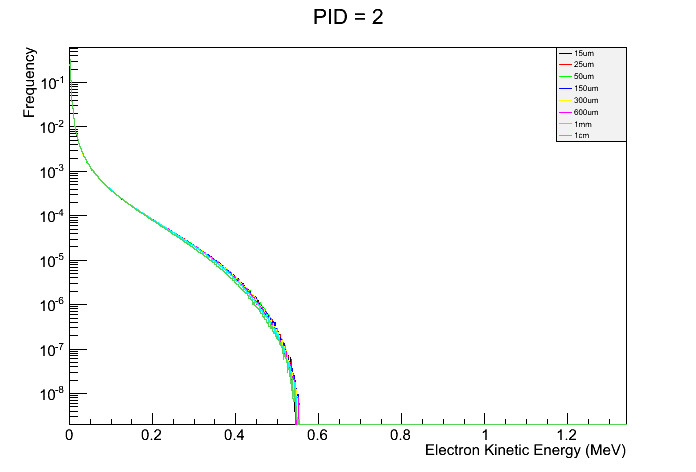
\includegraphics[width=\figurewidth]{Co60_PID2_SecElectron}
        \caption{Second Secondary Electron}
    \end{subfigure}
    \caption{Simulated kinetic energies of electrons from \iso{Co}{60} interactions}
    \label{fig:SecElecKinEDist}
\end{figure}
